\documentclass{article}
\usepackage{amsmath}
\usepackage{pdfpages}
\usepackage{xeCJK}
\usepackage{hyperref}
\usepackage{listings}
\lstset{
 columns=fixed,       
 numbers=left,                                        % 在左侧显示行号
 numberstyle=\tiny\color{gray},                       % 设定行号格式
 frame=single,                                          % 不显示背景边框
 keywordstyle=\color[RGB]{40,40,255},                 % 设定关键字颜色
 numberstyle=\footnotesize\color{darkgray},           
 commentstyle=\it\color[RGB]{0,96,96},                % 设置代码注释的格式
 stringstyle=\rmfamily\slshape\color[RGB]{128,0,0},   % 设置字符串格式
 showstringspaces=false,                              % 不显示字符串中的空格
 language=c++,                                        % 设置语言
}
\newcommand{\paper}[2]{\hyperlink{./papers/#1.pdf.#2}{(P#2)}}
\newcommand{\book}[2]{\href[page=#2]{./books/#1.pdf}{(P#2)}}


\title{Near-Data Processing}
\author{陈辉}
\date{}
\begin{document}
\maketitle
\tableofcontents
\newpage
\part{文献}
\section{\textit{Evolution-Strategies-as-a-Scalable-Alternative-to-Reinforcement-Learning}}
\paper{Evolution-Strategies-as-a-Scalable-Alternative-to-Reinforcement-Learning}{1}
\section{\textit{NEAR-DATA-PROCESSING-FOR-MACHINE-LEARNING}}
\paper{NEAR-DATA-PROCESSING-FOR-MACHINE-LEARNING}{1}

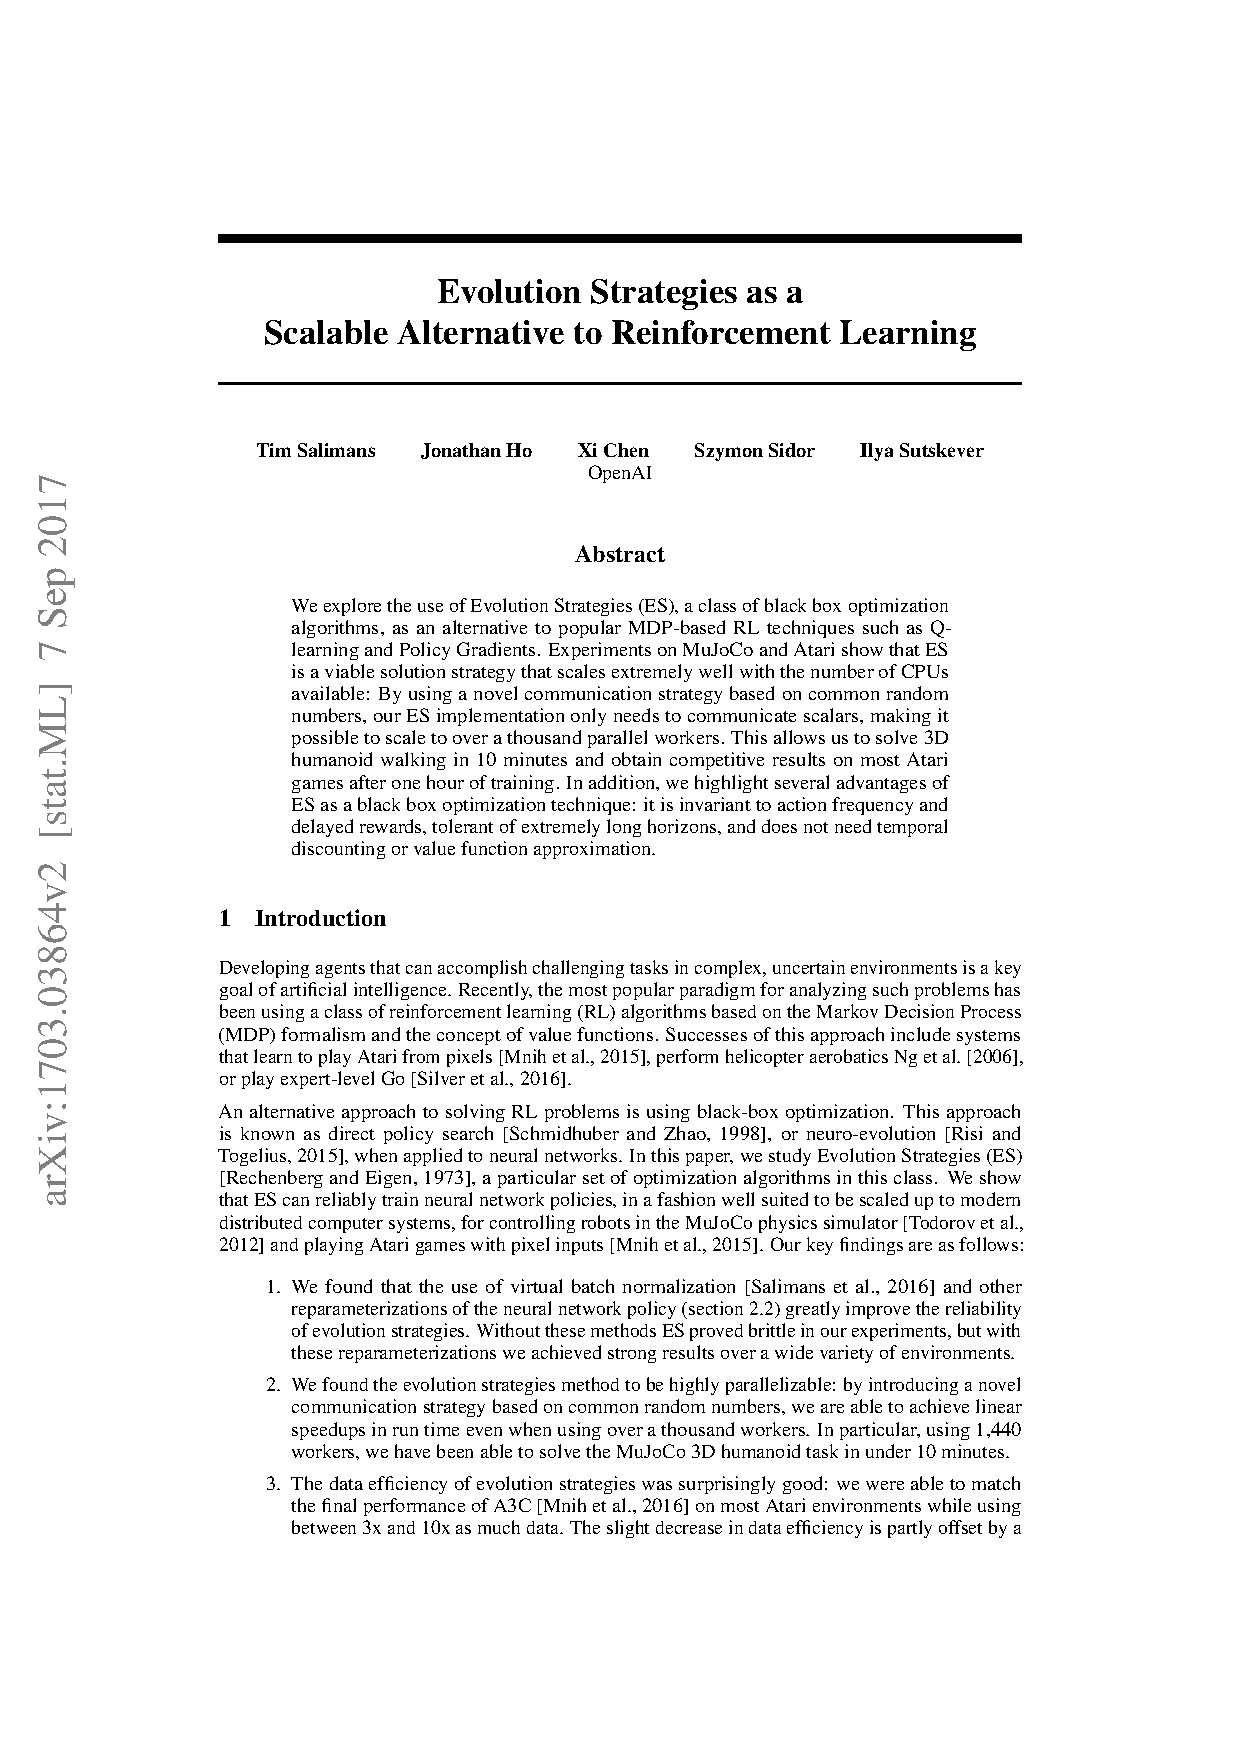
\includepdf[link=true,pages=-,fitpaper]{./papers/Evolution-Strategies-as-a-Scalable-Alternative-to-Reinforcement-Learning.pdf}



%\includepdf[link=true,pages=-,fitpaper]{./papers/<++>.pdf}
%\includepdf[link=true,pages=-,fitpaper,angle=-90]{./papers/<++>.pdf}

\end{document}
